\documentclass[pdf,aspectratio=169]{beamer}
\usepackage[]{hyperref,graphicx,siunitx,lmodern,booktabs}
\mode<presentation>{\usetheme{Astro}}

\graphicspath{ {../Images/} }

\sisetup{per-mode=symbol}

%preamble
\title{Banana for Scale}
\date{August 27, 2018}
\author{Jed Rembold}

\begin{document}

\begin{frame}{Welcome to Physics 110!}
  \begin{itemize}
	\item You have found your way to Phys 110: Astronomy!
	\item If you are in Lab Group A, we \alert{are} meeting for lab this week!
	\item Things to do before next class:
	  \begin{itemize}
		  \item Access the course page at \url{http://www.willamette.edu/~jjrembold/classes/wu110/main/}
		\item Read over the syllabus
		\item Get yourself a copy of the digital book
		\item Remember your phone or computer for polling questions on Wednesday
	  \end{itemize}
	\item WebWorK Assignment 1 is posted and due Wednesday
		\begin{itemize}
			\item Instructions and web address for logging in on the class website
		\end{itemize}
  \end{itemize}
\end{frame}

\begin{frame}{My Vitals}
  \begin{itemize}
	\item Name: Jed Rembold
	\item Office: Collins 311 (it's shared)
	\item Office Hours: M,W,Th 2-4pm \emph{and open door} ($\approx$always)
	\item Goudy Hours: M--Th 1-2pm near the windows in Goudy Commons
	\item Email: jjrembold@willamette.edu
	\item Phone: 503-370-6860
  \end{itemize}
\end{frame}

\begin{frame}{Grading}
  Attendance is mandatory for both lecture and labs!
  \begin{table}
	\centering
	\small
	\begin{tabular}{ccccc}
	  \toprule
	  Attendance & Lab & Homework & 3 Midterms & Final \\
	  \midrule
	  5\% & 20\% & 25\% & 30\% & 20\% \\
	  \bottomrule
	\end{tabular}
  \end{table}
\end{frame}

\begin{frame}{Attendance}
  %\begin{columns}
	%\column{.5\textwidth}
	\begin{itemize}
	  \item Class attendance is graded through participation in class polls
	  \item Generally 1-3 polls per day
	  \item Answering at all gets you full points for the day
	  \item Answering correctly gets you bits of extra credit
	  \item \url{http://rembold-class.ddns.net}
	  \item Will start on Wednesday
	\end{itemize}
	%\column{.5\textwidth}
	%\begin{center}
	  %\input{../Images/polling_qr}
	%\end{center}
  %\end{columns}
\end{frame}

\begin{frame}{Homework}
  \begin{itemize}
	  \item Homework will predominantly be online through \alert{\href{https://secure.willamette.edu/webwork2/Physics110/}{WebWorK}}
	\item Small assignments will be given after each class, to be due before the start of the next class
	\item You can do the assignments late, but will be only receive 75\% credit
	\item Don't be confused by WebWorK's terms
		\begin{itemize}
			\item Reduced Scoring Period: is the time when it is technically due (the next class period)
			\item Due date: is the point at which you can no longer receive \alert{any} credit for the assignment
		\end{itemize}
  \end{itemize}
\end{frame}

\begin{frame}{Tests}
  \begin{itemize}
	\item 3 Midterms
	  \begin{itemize}
		\item Test 1: Sep 28 - Chapters 1-6
		\item Test 2: Oct 26 - Chapters 7-14
		\item Test 3: Nov 16 - Chapters 15-24
	  \end{itemize}
	\item Final
	  \begin{itemize}
		\item Dec 12: 8:00-11:00am
		\item Will be comprehensive
	  \end{itemize}
	\item \alert{You will want access to at least a basic scientific calculator for test days, as you can't use your phone calculator for tests!}
  \end{itemize}
\end{frame}

\begin{frame}{Labs}
  \begin{itemize}
	\item Labs will be Monday from 7-10pm
	\item You \emph{must} be at lab in order to receive credit
	\item Groups A and B will alternate weeks for lab
		\begin{itemize}
			\item The schedule is posted on the webpage if you ever lose track!
		\end{itemize}
	\item I will post each week's lab manual on the website. You are responsible for printing it off and bringing it with you to lab.
	\item Labs will be a mix of observation activities (when weather allows), planetarium software demonstrations, and other activities
	\item Let me know as soon as possible if you are going to need to miss a lab
	  \begin{itemize}
		\item May be able to have you work through it at the other group's date
		\item May be able to make it up at a later week in the semester
	  \end{itemize}
  \end{itemize}
\end{frame}

\begin{frame}{Campuswire}
	\begin{itemize}
		\item Invitations to Campuswire should be going out today
		\item Classroom forum to better communication and asking of questions
		\item Asking questions there allows others to benefit from seeing my (or other students!) responses
		\item I will also use it for general communication and some occassional polling, so check it out!
	\end{itemize}
\end{frame}

\begin{frame}{Astronomy}
  \begin{center}
	\includegraphics[width=.7\linewidth]{ch1_astronomy.jpg}
  \end{center}
\end{frame}


\begin{frame}{Some Basics}
  \begin{itemize}
	\item Distances
	  \begin{itemize}
		\item Meters instead of feet
		\item Kilometers instead of miles
		\item Astronomical Units (AU)
		  \begin{itemize}
			\item Average distance from Earth to Sun
			\item $\approx$ 150 million km
		  \end{itemize}
		\item Light-year
		  \begin{itemize}
			\item Distance light travels in a year
			\item $\approx$ 10 trillion km
			\item A light-year is a \alert{distance} not a time!
		  \end{itemize}
	  \end{itemize}
	\item Times
	  \begin{itemize}
		\item Still use seconds, days, years, etc
	  \end{itemize}
  \end{itemize}
\end{frame}

\begin{frame}{Recall Your SI Notation!}
  \begin{table}
	\centering
	\begin{tabular}{lcccl}
	  \toprule
	  $10^n$ & Prefix & Symbol & Scale \\
	  \midrule
	  $10^{-2}$ & centi & c & Hundredth & 0.01 \\
	  $10^0$ & & & One  & 1\\
	  $10^3$ & kilo & k & Thousand & 1000 \\
	  $10^6$ & mega & M & Million & 1000000 \\
	  $10^9$ & giga & G & Billion & 1000000000\\
	  $10^{12}$ & tera & T & Trillion & 1000000000000 \\
	  \vdots & \vdots & \vdots &\vdots & \vdots \\
	  \bottomrule
	\end{tabular}
  \end{table}
\end{frame}

\begin{frame}{What does this look like?}
  \href{http://htwins.net/scale2/}{\includegraphics[width=\textwidth]{ch1_ScalePic.png}}
\end{frame}

\begin{frame}{The Implications of Light Speed}
  \begin{itemize}
	\item Light travels at a constant, fast speed (\SI{3e8}{\meter\per\second})
	\item Astronomic distances so large though that light takes measurable time to reach us
	\item Looking at distant objects is really looking back in time
  \end{itemize}
  \begin{figure}[h!]
	\centering
	\includegraphics[width=\textwidth]{ch1_TimeAndDistance.jpg}
  \end{figure}
\end{frame}

\begin{frame}{Solar System Sizes}
  \centering
  \setbeamercovered{invisible}
  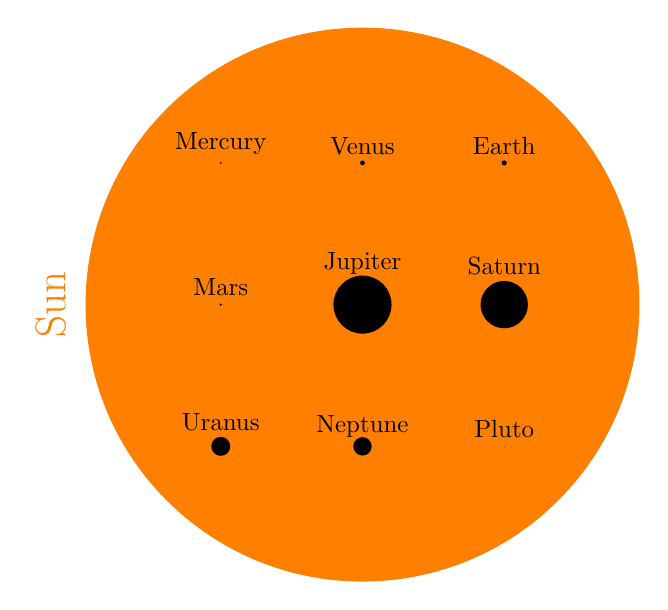
\begin{tikzpicture}[scale=0.9, transform shape]
	\draw[orange,fill=orange] (0,0) circle(3.9cm);
	\node[orange,rotate=90] at (-4.4,0) {\LARGE Sun};\pause
	\fill[black] (-2,2) circle(0.13mm) node[above] {Mercury};
	\fill[black] (-0,2) circle(0.34mm) node[above] {Venus};
	\fill[black] (2,2) circle(0.36mm) node[above] {Earth};
	\fill[black] (-2,0) circle(0.19mm) node[above] {Mars};\pause
	\fill[black] (-0,0) circle(4.1mm) node[above,yshift=3mm] {Jupiter};
	\fill[black] (2,0) circle(3.34mm) node[above,yshift=3mm] {Saturn};
	\fill[black] (-2,-2) circle(1.34mm) node[above,yshift=1mm] {Uranus};
	\fill[black] (-0,-2) circle(1.3mm) node[above] {Neptune};\pause
	\fill[black] (2,-2) circle(0.06mm) node[above] {Pluto};
	\onslide<1->
  \end{tikzpicture}
\end{frame}

\begin{frame}{Extrasolar Sizes}
  \begin{itemize}
	\item Our own Solar System seems huge enough
	\item Space \emph{really} kicks in once we leave our system
	  \begin{itemize}
		\item Nearest star (Alpha Centauri) is $\approx$8000x the distance to Pluto
		\item This is a common star separation distance in the Milky Way
		\item The Milky Way has has many stars as all the grains of dry sand on all Earth's beaches
		\item With the Milky Way shrunk to the scale of a football field, the entire Solar System would be a microscopic dot on roughly the 20 yard line
		\item The Milky Way is just one of $\approx$100 billion galaxies that we've seen in the observable universe
	  \end{itemize}
  \end{itemize}
  \begin{alertblock}{Moral of the Story}<2>
	Space is big. Like, unbelievably gigantic big. Stupidly big.
  \end{alertblock}
\end{frame}

\begin{frame}{A Universal Timeline}
	\begin{itemize}[<+->]
	\item Let's shrink the entire history of the Universe into a single year
	  \begin{itemize}
		\item Jan 1 - The Big Bang
		\item Feb - The Milky Way forms
		\item Sept 3 - Earth forms
		\item Sept 22 - Life begins on Earth
		\item Dec 26 - Dinosaurs rise up
		\item Dec 30 - Dinosaurs extinct
		\item On Dec 31:
		  \begin{itemize}
			\item 9pm - Early apes evolve
			\item 11:58pm - Modern Humans evolve
			\item 11:59:49pm - Pyramids built
			\item 11:59:59pm - Discover that the Earth orbits the Sun
		  \end{itemize}
	  \end{itemize}
	\item Humans have been around for 0.0004\% the history of the universe
	\item Check out ``History of the Universe'' by Halycon in the app store on your phone!
  \end{itemize}
\end{frame}

\begin{frame}{Movement: Motion within Motion within\ldots}
  Small to Big:
  \begin{itemize}
	\item Earth rotates on it's axis each 24 hours
	\item Earth rotates around the Sun in 365.25 days
	\item The Sun rotates around the center of the Milky Way in $\approx$230 million years
	\item We also have random and erratic bits of movements from local effects (nearby planets, stars, galaxies etc)
	\item All galaxies are moving away from each other due to the universe expanding
	  \begin{itemize}
		\item Raisin cake analogy
	  \end{itemize}
  \end{itemize}
\end{frame}

\begin{frame}{Takeaways}
  \begin{alertblock}{Distance}
	Compared to us, the universe is nearly unimaginably large
  \end{alertblock}
  \begin{alertblock}{Time}
	Our lives are an indistinguishable speck in the age of the universe
  \end{alertblock}
  \begin{alertblock}{Movement}
	Literally everything is undergoing some sort motion. Both organized (orbits) and chaotic (pushes and pulls from neighbors).
  \end{alertblock}
\end{frame}

\begin{frame}{PSA: Calculator Advice}
  \begin{itemize}
	\item Remember your order of operations!
	  \begin{itemize}
		\item Parenthesis, Exponents, Mult/Div, Add/Sub
		\item Don't forget parenthesis when dividing by multiple things! (But don't go overboard with parenthesis either, or things get confusing!)
	  \end{itemize}
	\item Lots of large or tiny numbers in this class
	  \begin{itemize}
		  \item \num{6e8} = \texttt{\fbox{6} \fbox{$\times$} \fbox{10\^{}} \fbox{8}} = \texttt{\fbox{6} \fbox{EE} \fbox{8}}
		\item Most calculators will return values in \texttt{E} notation
		  \begin{figure}[h!]
			\centering
			\includegraphics[width=7cm]{ch1_iphoneCalc.png}
		  \end{figure}
	  \end{itemize}
  \end{itemize}
\end{frame}





\end{document}
